\section{Intelligence Artificielle Aléatoire}

Notre Intelligence Artificielle va devoir s'expandre et se développer, nous allons donc dans un premier temps effectuer aléatoirement les actions liées aux vaisseaux puis celles liées aux systèmes.
Dans un premier temps, la stratégie pour les vaisseaux suit simplement le diagramme suivant :

\begin{figure}[!h]
\centering
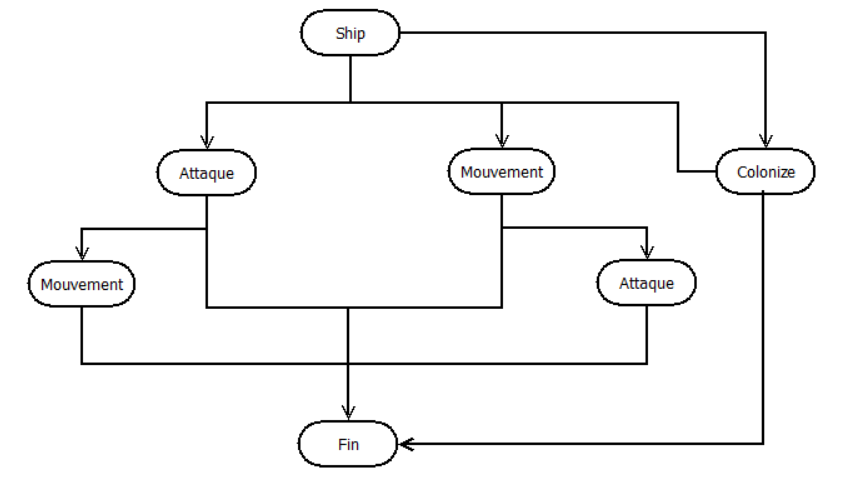
\includegraphics[width=1\textwidth]{pics/IA_random.PNG}
\caption[Stratégie d'expansion]{\label{figure_simple}Stratégie d'expansion}
\end{figure}



\begin{itemize}
\item L'IA va sélectionner un vaisseau,
\item Elle va ensuite choisir aléatoirement une action parmi les 3 disponibles sachant que l'action de coloniser à une probabilité plus élevé que les deux autres,
\item Selon l'action qu'elle a effectué elle pourra déplacer ou attaquer, si elle choisit la commande de colonisation et qu'elle est possible le vaisseau est alors détruit sinon on teste les commandes d'attaque et de déplacement,
\item Finalement si il reste des vaisseaux disponible, on recommence le même paterne 
\end{itemize}

Dans un second temps, la stratégie de développement des systèmes et la suivante : 

\begin{figure}[!h]
\centering
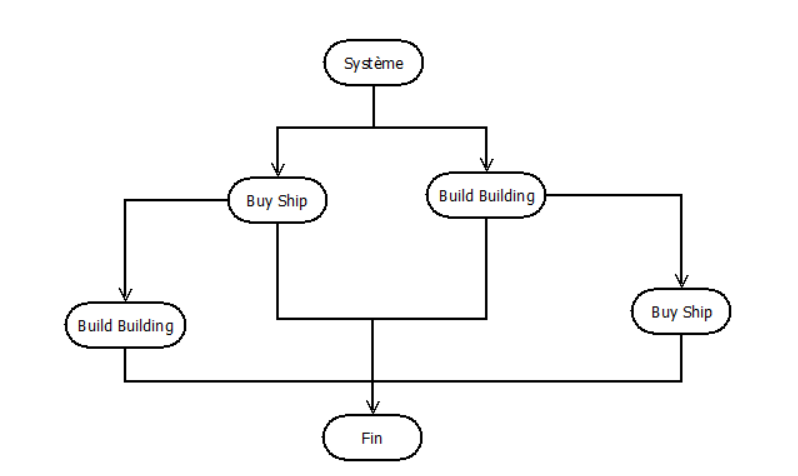
\includegraphics[width=1\textwidth]{pics/IA_random2.PNG}
\caption[Stratégie de développement]{\label{figure_simple}Stratégie de développement}
\end{figure}

\begin{itemize}
\item L'IA va sélectionner un système,
\item Elle va alors choisir aléatoirement entre construire un bâtiment ou acheter un vaisseau,
\item Si une commande est effectuée, on passe à un autre système disponible sinon on test l'autre commande,
\item Finalement on passe à un autre système disponible
\end{itemize}

\section{Intelligence Artificielle Heuristique}

Nous allons maintenant voir l'IA heuristique qui va prendre de meilleurs décisions que l'IA aléatoire. Nous avons implémenter des poids sur certaines commandes en fonction de sa situation actuelle et celle de l'adversaire.
Pour la partie expansion. Un vaisseau n'attaquera plus les vaisseaux qui ont un avantages sur lui, il favorisera la colonisation de nouveaux systèmes
Pour la partie développement, cela dépendra principalement de la flotte de l'adversaire :\\

\begin{itemize}
    \item Si l'IA possède une flotte de vaisseaux qui ont l'avantage sur celle de l'adversaire, l'IA va alors préférer la construction de nouveau bâtiment pour augmenter sa production de ressources. 
    \item Si la flotte de l'IA est plus faible que celle de l'adversaire, l'IA va alors favoriser l'achat de vaisseaux qui contre la flotte actuelle de l'adversaire.
\end{itemize}
